\documentclass[14pt,a4paper,article]{ncc}
\usepackage[a4paper, mag=1000, left=2.5cm, right=1cm, top=2cm, bottom=2cm, headsep=0.7cm, footskip=1cm]{geometry}
\usepackage[utf8]{inputenc}
\usepackage[T2A]{fontenc}
\usepackage[english,russian]{babel}
\usepackage{indentfirst}
%\usepackage[dvipsnames]{xcolor}
\usepackage{amsfonts} 
\usepackage{amssymb} 
\usepackage{amsmath, etoolbox}
\usepackage{graphicx}
\usepackage{float}
\graphicspath{{../figure/}}
\DeclareGraphicsExtensions{.png,.jpg, .jpeg}

%\bibliographystyle{gost-numeric.bbx}
\usepackage{csquotes}
\usepackage[backend=biber]{biblatex}
\addbibresource{literature.bib}

\usepackage{fancyhdr}
\pagestyle{fancy}
\fancyhead[LE,RO]{\thepage}
\fancyfoot{} 

\usepackage{listings}

%\patchcmd\subequations
%{\theparentequation\alph{equation}}
%{\subequationsformat}
%{}{}

%\newcommand{\subequationsformat}{\theparentequation.\arabic{equation}}

%\numberwithin{equation}{subsection}


\usepackage[colorlinks]{hyperref}
\hypersetup{linkcolor=black}

\begin{document}

% Title page 
\begin{titlepage}
    \begin{center}
        \textsc{
            Санкт-Петербургский политехнический университет Петра Великого \\[5mm]
            Физико-механический институт\\[2mm]
            Высшая школа прикладной математики и вычислительной физики
        }   
        \vfill
        \textbf{\large
            Компьютерные сети\\
            Отчёт по лабораторной работе №2 \\
            ``Задача византийских генералов'' \\[3mm]
            %по курсовой работе \\[3mm]
        }                
    \end{center}

    \vfill
    \hfill
    \begin{minipage}{0.5\textwidth}
        Выполнил: \\[2mm]   
		Студент: Дамаскинский Константин \\
		Группа: 5040102/10201\\
    \end{minipage}

	\hfill
	\begin{minipage}{0.5\textwidth}
		Принял: \\[2mm]
		к. ф.-м. н., доцент \\   
		Баженов Александр Николаевич
	\end{minipage}

    \vfill
    \begin{center}
        \theyear\ г.
    \end{center}
\end{titlepage}

\tableofcontents
%\listoffigures
%\listoftables
\newpage

\section{Постановка задачи}
Пусть дано $n$ генералов, $m$ из которых византийские. Каждый генерал в начале располагает неким значением $v_i$, не известным другим генералам. Требуется разработать протокол взаимодействия, в результате следования которому каждый невизантийский генерал сформирует набор значений $\{u_i\}, i = \overline{1,n}$. Сформированный набор значений должен совпадать у всех генералов, при этом для индексов $i$, соответствующих невизантийским генералам, $u_i$ должно совпадать с $v_i$.
Будем считать, что каналы связи являются надёжными, а сообщения невозможно подделать.
Необходимо реализовать алгоритм Лампорта-Шостака-Пиза для решения задачи византийских генералов.

\section{Теория}
Генералы будут общаться по протоколу, соответствующему частному случаю алгоритма Лампорта-Шостака-Пиза. Обмен сообщениями будет происходить в 2 этапа:
\begin{itemize}
	\item На первом этапе каждый генерал передаёт всем остальным одно значение, при этом невизантийские генералы честно передают своё значение $v_i$, а византийские могут передавать произвольное значение (при этом он может передавать разным генералам разные значения). В результате у каждого генерала образуется вектор значений, пришедших ему от остальных
	\item На втором этапе каждый невизантийский генерал передаёт всем остальным вектор значений, сформированный на первом этапе, а византийский – вектор произвольных значений (потенциально различных для различных генералов)
\end{itemize}
    
В результате у каждого генерала формируется матрица информации, состоящая из вектора, сформированного на первом этапе, и векторов, полученных на втором этапе.
Таким образом у генерала про каждого союзника формируется набор из нескольких (потенциально различных) значений. В качестве итогового значения, генерал выбирает наиболее часто встречающееся в наборе. Если таких значений несколько, то итоговое значение считается неопределенным.
Алгоритм Лампорта-Шостака-Пиза гарантирует, что следуя его протоколу генералы всегда смогу прийти к консенсусу, в случае если $n > 3m$.

\section{Реализация}
Модель реализована на языке программирования Python. Все генералы работают в отдельных потоках, создаваемых с использованием модуля threading. Также в отдельных потоках работают все 3 каналы связи между генералами. Для обеспечения потокобезопастности каналов используются mutex (класс Lock из модуля threading). При переходе к следующему этапу алгоритма установлены точки барьерной синхронизации для всех генералов (класс Barrier из модуля threading).

На канальном уровне генералы общаются с помощью протокола SRP. Сетевой уровень для данной задачи тривиален, так как по условию предполагается, что канал связи существует между любой парой генералов. 


\section{Результаты}
Оценку эффективности протоколов будем проводить по двум
параметрам:

\begin{itemize}
	\item коэффициент эффективности $k$ -- количество всех пакетов / количество переданных пакетов
	\item время от начала до конца передачи в секундах – $t$
\end{itemize}

Для оценки эффективности была проведена серия экспериментов с
различными значениями размера окна и вероятности потери пакетов. Во всех
тестах количество передаваемых пакетов равно 100, timeout = 0.2 с.

Зависимость коэффициента эффективности $k$ и времени передачи $t$ от
вероятности потери пакета $p$ при фиксированном размере окна
window\_size = 3 представлена в таблице 1 и графически на рис. 4.

\begin{figure}[H]
	\begin{center}
		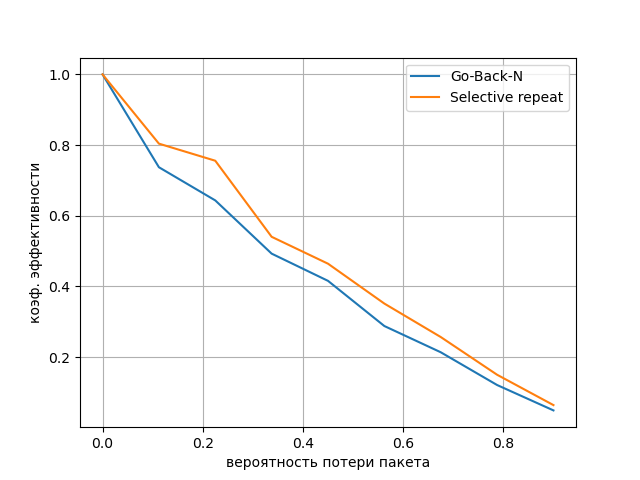
\includegraphics[scale=0.5]{fig1}
		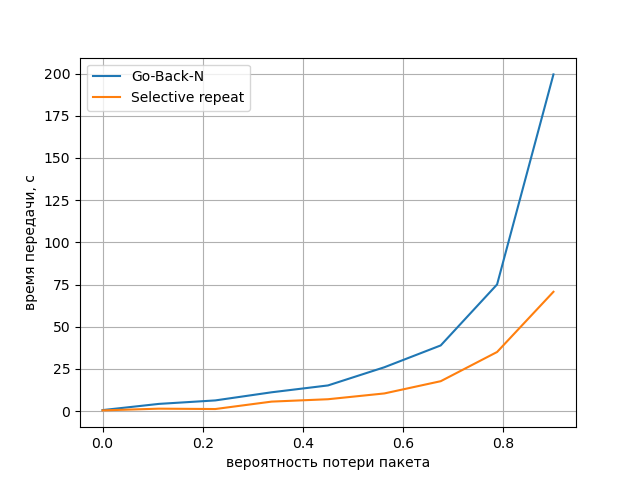
\includegraphics[scale=0.5]{fig2}
		\caption{Визуализация передачи данных с использованием скользящего окна}
	\end{center}
\end{figure}

\begin{table}[H]
	\begin{center}
		\begin{tabular}{|c|c|c|c|c|}
			\hline
			 & \multicolumn{2}{c|}{Go-Back-N} & \multicolumn{2}{c|}{Selective Repeat} \\
			\hline
			$p$ & $k$ & $t$ & $k$ & $t$ \\
			\hline
			0.0 & 0.55 & 1.00 & 0.37 & 1.00 \\
			\hline
			0.1 & 4.23 & 0.74 & 1.40 & 0.80\\
			\hline
			0.2 & 6.29 & 0.64 & 1.18 & 0.76\\
			\hline
			0.3 & 11.11 & 0.49 & 5.59 & 0.54\\
			\hline
			0.5 & 15.17 & 0.42 & 6.99 & 0.46\\
			\hline
			0.6 & 25.95 & 0.29 & 10.43 & 0.35\\
			\hline
			0.7 & 38.89 & 0.21 & 17.68 & 0.26\\
			\hline
			0.8 & 75.04 & 0.12 & 35.00 & 0.15\\
			\hline
			0.9 & 199.54 & 0.05 & 70.68 & 0.06\\
			\hline
		\end{tabular}
		\caption{ Зависимость эффективности протоколов от вероятности потери пакета при window\_size = 3}
	\end{center}
\end{table}


Зависимость
эффективности $k$ и времени передачи $t$ от размера окна window\_size при
заданной вероятности потери пакета $p = 0.3$ представлена в табл. 2 и на рис. 5.

\begin{figure}[H]
	\begin{center}
		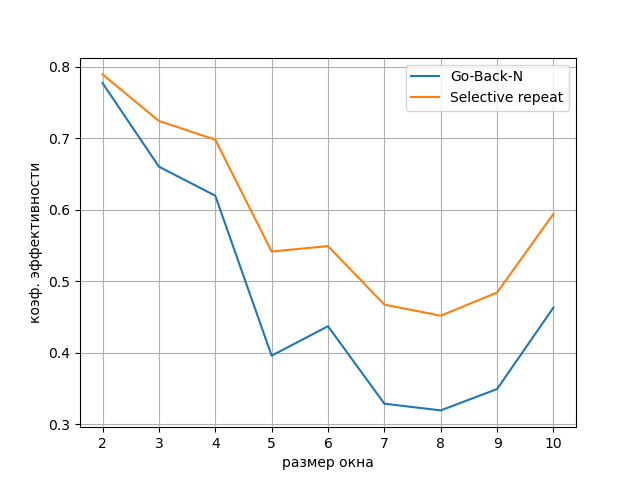
\includegraphics[scale=0.52]{fig3}
		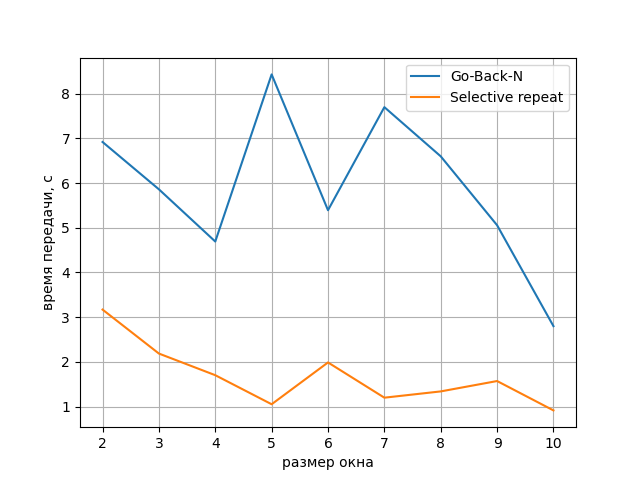
\includegraphics[scale=0.52]{fig4}
		\caption{Зависимость коэффициента эффективности и времени передачи от размера окна при $p = 0.3$}
	\end{center}
\end{figure}

\begin{table}[H]
	\begin{center}
		\begin{tabular}{|c|c|c|c|c|}
			\hline
			& \multicolumn{2}{c|}{Go-Back-N} & \multicolumn{2}{c|}{Selective Repeat} \\
			\hline
			window size & $k$ & $t$ & $k$ & $t$ \\
			\hline
			2 & 6.92 & 0.78 & 3.17 & 0.79 \\
			\hline
			3 & 5.86 & 0.66 & 2.19 & 0.72\\
			\hline
			4 & 4.69 & 0.62 & 1.70 & 0.70\\
			\hline
			5 & 8.43 & 0.40 & 1.05 & 0.54\\
			\hline
			6 & 5.39 & 0.44 & 1.99 & 0.55\\
			\hline
			7 & 7.70 & 0.33 & 1.20 & 0.47\\
			\hline
			8 & 6.60 & 0.32 & 1.34 & 0.45\\
			\hline
			9 & 5.06 & 0.35 & 1.57 & 0.48\\
			\hline
			10 & 2.80 & 0.46 & 0.91 & 0.59\\
			\hline
		\end{tabular}
		\caption{Зависимость эффективности протоколов от вероятности потери пакета при window\_size = 3}
	\end{center}
\end{table}


\section{Обсуждение}
В результате работы реализован алгоритм Лампорта-Шостака-Пиза для решения частного случая задачи Византийских генералов. Показана работоспособность алгоритма для $n = 5$ честных генералов и $m = 1$  византийского генерала среди них. Реализована модель взаимодействия между генералами (независимыми узлами) на сетевом и канальном уровне. Для обеспечения корректной работы параллельного алгоритма были использованы различные примитивы синхронизации.

\printbibliography
%\addcontentsline{toc}{section}{Литература}

\section{Приложения} \label{app}

\begin{enumerate}
	\item Репозиторий с кодом программы и кодом отчёта:
	
	\href{https://github.com/kystyn/networks}{https://github.com/kystyn/networks}

\end{enumerate}


\end{document}
